% !TEX root = ../../semexp-thesis.tex

\section{Toward a Semantic Toolset for Exploratory Programming}
\label{sec:application/system}

In the following, we describe another application of semantic conversations that aims at a broader adoption of semantic tools in exploratory programming systems.
Our approach is based on the observation that many exploratory programming systems employ \emph{object-oriented user interfaces}.
An object-oriented user interface (OOUI) is a---predominantly graphical---type of user interface that employs an object-oriented metaphor and an injective mapping from (complex) domain objects to visual elements~\cite{collins1995designing}.
Examples of OOUIs can be found in several domains, including graphical editors such as Microsoft PowerPoint, project management software such as Jira, and also several programming environments such as Eclipse, Scratch, or Smalltalk systems~\cite{pawson2001naked}.

\begin{figure}
	\centering
	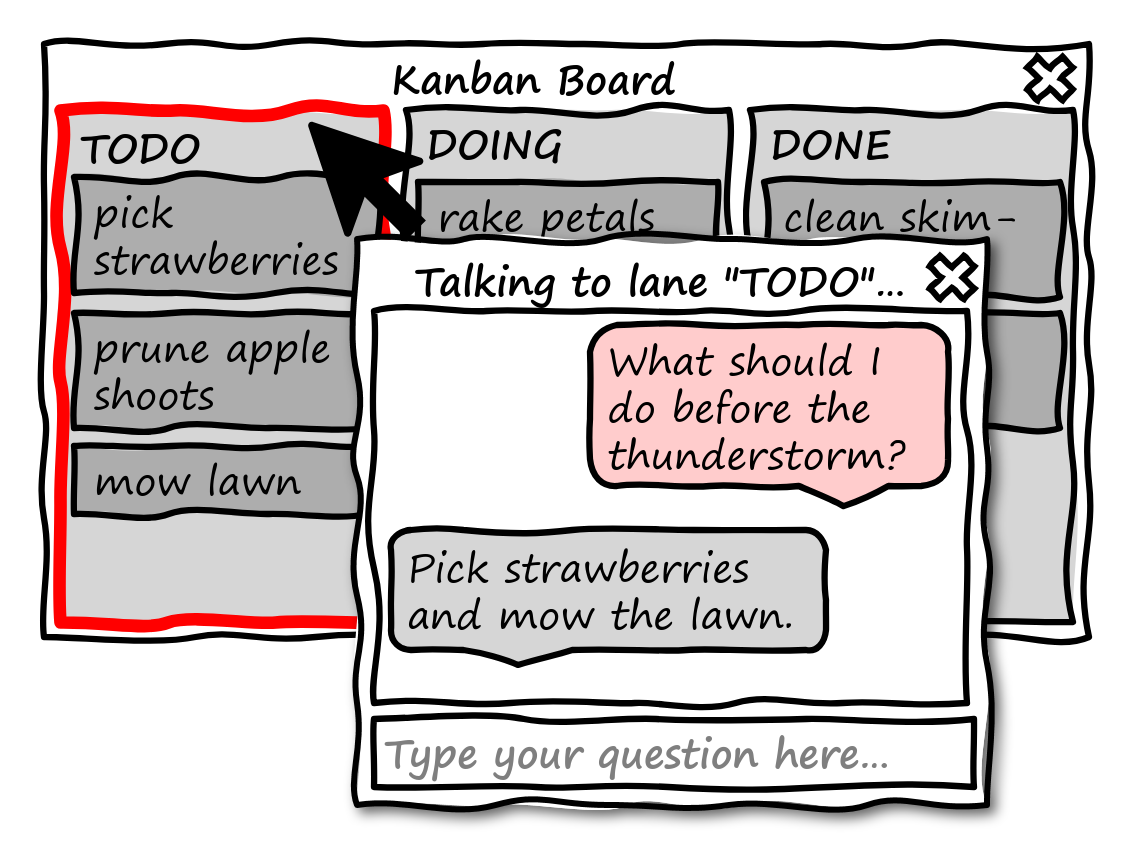
\includegraphics[height=12\baselineskip]{chapters/08_application/03_system/project.png}
	\caption[Sketching a generic integration of semantic object interfaces into object-oriented user interfaces.]{
		Through the generic integration of semantic object interfaces into object-oriented user interfaces, users can select arbitrary domain objects from the UI and start a natural-language conversation with them.
		Here, a user talks to a lane in a project management system to filter its items.
	}
	\label{fig:application/system/project}
\end{figure}

We propose a simple mechanism for OOUI frameworks that integrates semantic object interfaces with the visual mapping of OOUIs.
This allows users to select domain objects on their screen to talk to them in natural language.
At the same time, domain developers are not required to put manual effort into writing prompts or preparing contextual information for LLMs, as the agent still fetches all required information by itself through automated experiments.
For example, in a project management system that organizes task items in boards and lanes, a user could select a lane and ask for a semantic filtration or summary of the items it contains~(\cref{fig:application/system/project}).

We apply this concept to graphical, object-oriented programming systems such as Squeak"/Smalltalk, where tools such as code browsers, (projectional) editors, (back-in-time) debuggers, and profilers represent views on underlying code objects and their derived artifacts such as classes in packages, code blocks in methods, and call stacks or program traces.
In this way, programmers can chat with code objects to ask for the responsibilities or collaborators of a class~(\cref{fig:application/system/browser}), explain or refactor a code block~(\cref{fig:application/system/editor}), search for the origin of values or cause of state changes in a program stack or slice~(\cref{fig:application/system/debugger}), identify the bottlenecks in a program trace, and more.

\FloatBarrier

\begin{figure}[Z]
	\centering
	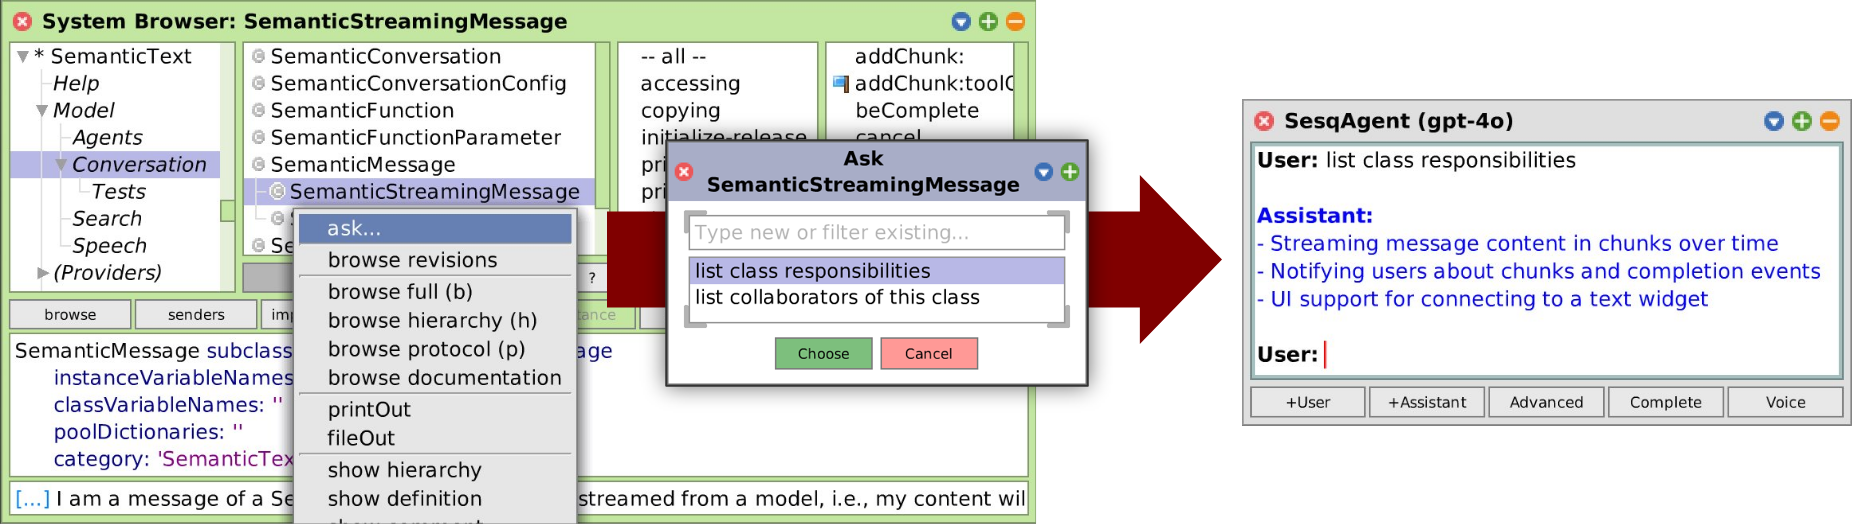
\includegraphics[width=\linewidth]{chapters/08_application/03_system/browser.png}
	\caption[In a semantic code browser, programmers can engage in natural-language conversations with classes to explore them, e.g., by asking for their responsibilities or collaborators.]{
		In a semantic code browser (here: the default system browser of Squeak 6.1Alpha), programmers can engage in natural-language conversations with classes to explore them, e.g., by asking for their responsibilities or collaborators.
	}
	\label{fig:application/system/browser}
\end{figure}

\begin{figure}[Z]
	\centering
	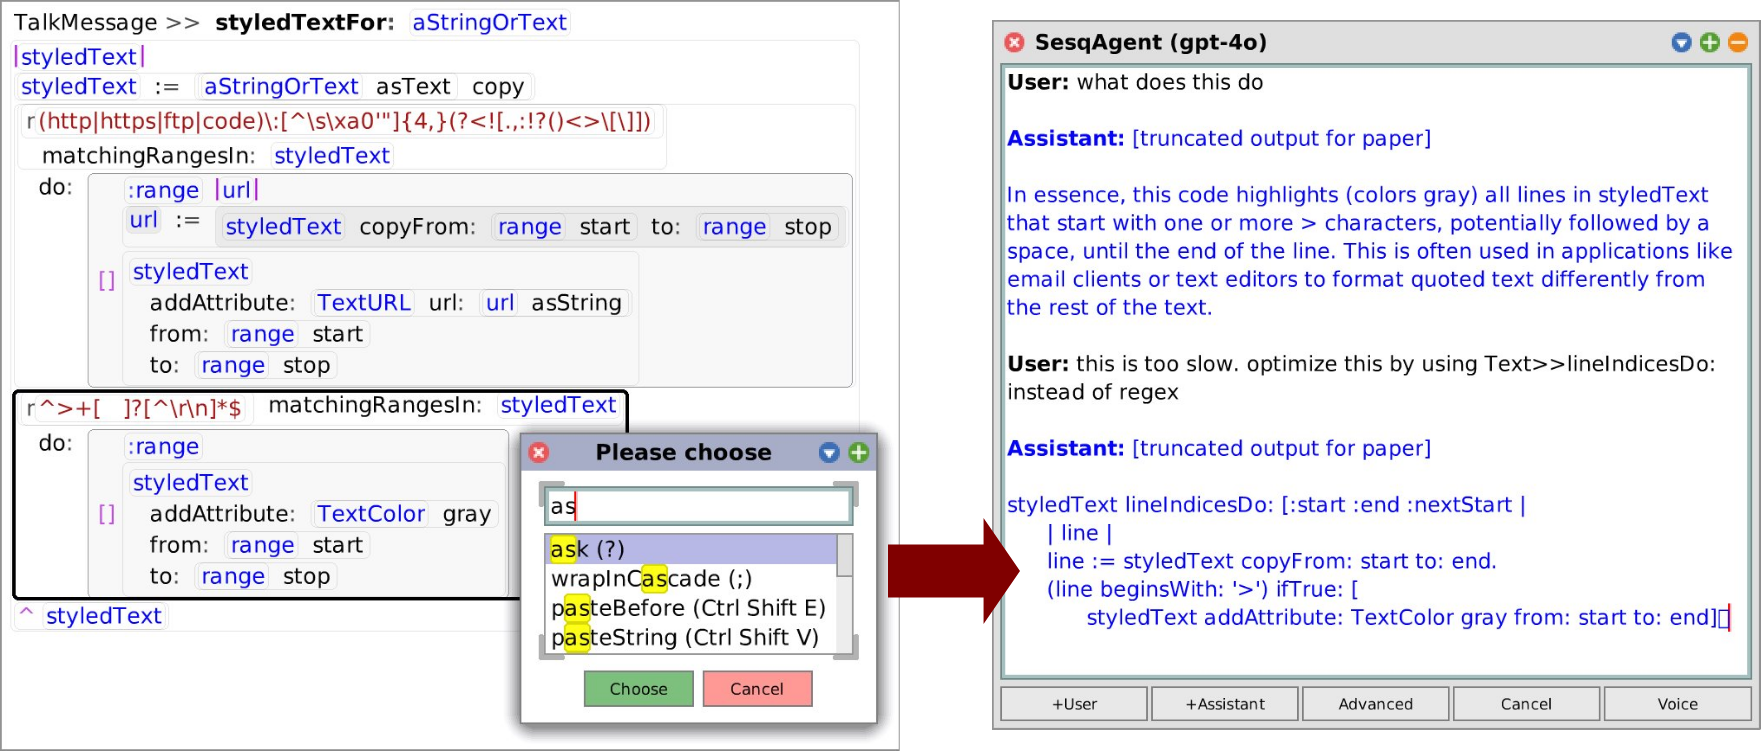
\includegraphics[width=\linewidth]{chapters/08_application/03_system/editor.png}
	\caption[In a semantic projectional editor, programmers can chat with single code blocks to explain, refactor, or execute them.]{
		In a semantic projectional editor (here: Sandblocks~\cite{beckmann2020visual}), programmers can chat with single code blocks to explain, refactor, or execute them.
	}
	\label{fig:application/system/editor}
\end{figure}

\begin{figure}[p]
	\centering
	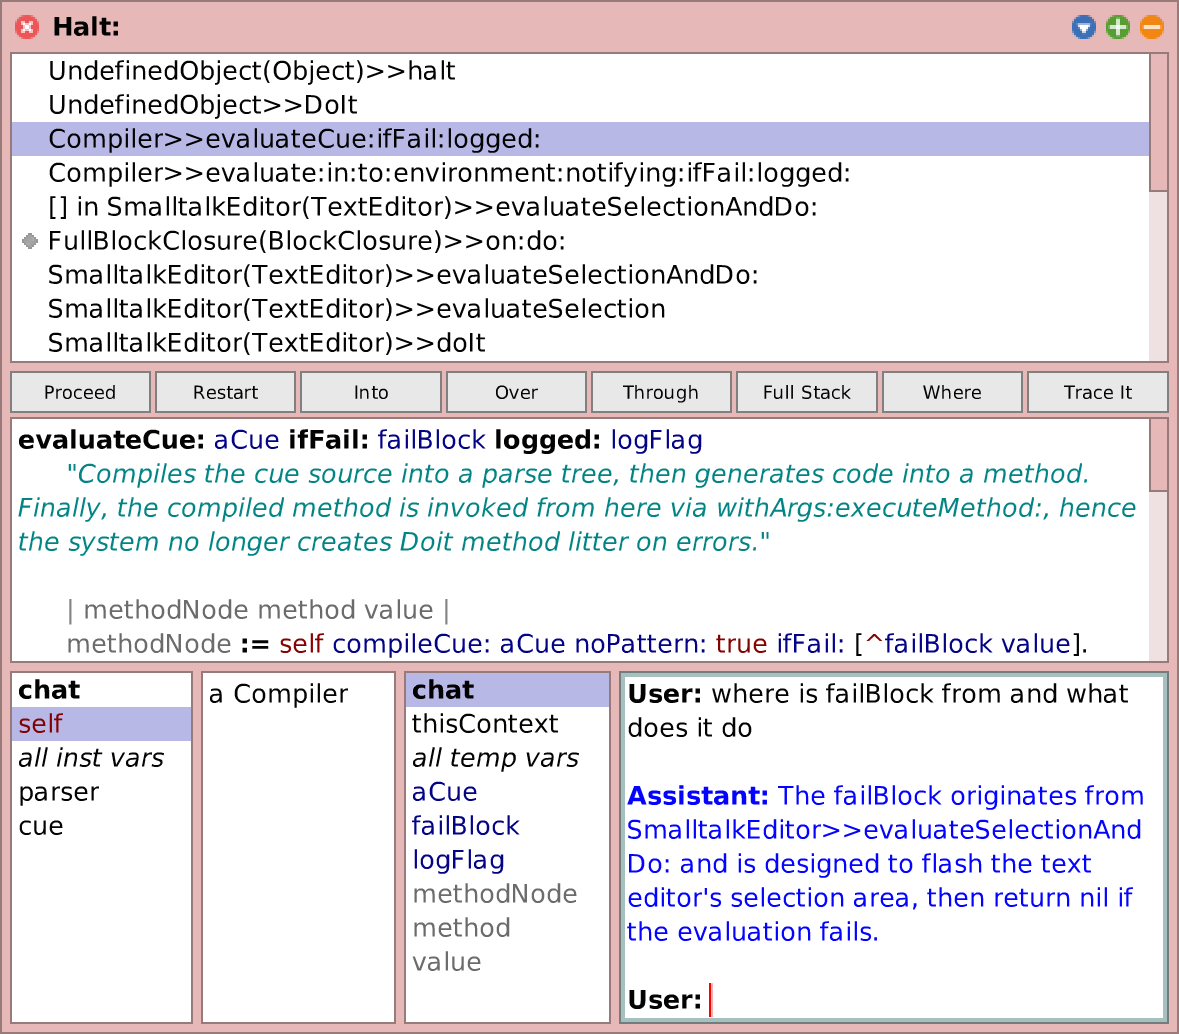
\includegraphics[width=0.9\textwidth]{chapters/08_application/03_system/debugger.png}
	\caption[In a semantic debugger, programmers can ask for the origin and meaning of values on the program stack.]{
		In a semantic debugger (here: the Squeak debugger), programmers can ask for the origin and meaning of values on the program stack.
	}
	\label{fig:application/system/debugger}
\end{figure}

Thus, we effectively upgrade existing programming tools to \emph{semantic tools} by extending them with a conversational interface for an agent that will autonomously explore the programming artifacts shown in a tool.
This allows programmers to express their questions and intents about programming artifacts in natural language and in the context of their exploratory session (which is captured in the conversation history of the agent).
While the efficacy of this approach still hinges on the advancements in LLM capabilities and the precision of prompt engineering, this integration into exploratory programming systems promises a noticeable reduction in semantic distance, thereby supporting programmers' conceptual focus and enhancing their interaction with systems at a high level of abstraction.

\FloatBarrier
